\documentclass[12pt]{article}
\usepackage{amssymb}
\usepackage{amsmath}
\usepackage[margin=1in]{geometry}
\usepackage{enumitem} 
\usepackage{graphicx}
\usepackage{lingmacros}
\usepackage{tree-dvips}
\usepackage{amsfonts}
\usepackage{xcolor}
\usepackage{mathrsfs}
\usepackage{indentfirst}
\usepackage{CJKutf8}
%\usepackage{amsmath}
\pagestyle{plain}

\begin{document}
\begin{CJK}{UTF8}{bsmi}

\section{Kinematics Analysis}
\begin{table}[h]
\centering
\caption{DHtable}
\label{tab:DHtable}
\begin{tabular}{ccccc} 
\hline \hline
	i	&$\alpha _{i-1}$	&$a_{i-1}$	&$\theta _i$			&$d_i$	\\\hline
	1   &0    				&0			&$\theta _1$			&135 \\
	2   &$-90^{o}$   		&0			&$\theta _2$			&0 \\
	3   &0    				&135		&$\theta _3$ 			&0 \\
	4   &$-90^{o}$    		&38			&$\theta _4$ 			&120 \\
	5   &$90^{o}$    		&0			&$\theta _5$ 			&0 \\
	6   &$-90^{o}$    		&0			&$\theta _6$ 			&70 \\
\end{tabular}
\end{table}
Denavit-Hartenberg parameters are shown as Table \ref{tab:DHtable}. Then, the forward kinematics of the robot arm is derived as
\begin{equation*}
\begin{split}
^0_6\text{T} =
\ ^0_1\text{T} \cdot ^1_2\text{T} \cdot ^2_3\text{T} \cdot ^3_4\text{T} \cdot ^4_5\text{T} \cdot ^5_6\text{T} =
\begin{bmatrix}
^0_6\text{R}_{3\times 3} 	&^0\vec{P}_{6org}\\
0_{1\times 3}				&1\\
\end{bmatrix}
\end{split}
\end{equation*}
Where $^0_6\text{R}_{3\times 3}$ is the rotation matrix between frame\{0\} and frame\{6\}, $^0\vec{P}_{6org}$ is the origin of the frame\{6\} observed from frame\{0\}
The detailed indexes is shown as Appendix \ref{appendix:forward}



\begin{equation*}
\begin{split}
J_{g6,20} =\  &S_4S_5(135S_2 + \sqrt{23961}cos(\theta _2 + \theta _3 - \tan ^{-1}(19/60)))\\
J_{g6,21} =\  &38C_5 + 135C_3C_5 + 120C_4S_5 - 135C_4S_3S_5\\
J_{g6,22} =\  &38C_5 + 120C_4S_5\\
J_{g6,23} =\  &
J_{g6,24} =\  
J_{g6,25} =\  0\\
J_{g6,30} =\  &C_2C_3S_4S_6 + C_2C_6S_3S_5 + C_3C_6S_2S_5 - S_2S_3S_4S_6 + \theta _2C_2C_3C_6S_5 + \theta _3C_2C_3C_6S_5 \\
			  &+ \theta _4C_2C_3C_4S_6 + \theta _5C_2C_5C_6S_3 + \theta _5C_3C_5C_6S_2 + \theta _6C_2C_3C_6S_4 - \theta _2C_2S_3S_4S_6\\
			  & - \theta _2C_3S_2S_4S_6 - \theta _2C_6S_2S_3S_5 - \theta _3C_2S_3S_4S_6 - \theta _3C_3S_2S_4S_6 - \theta _3C_6S_2S_3S_5\\
			  & - \theta _4C_4S_2S_3S_6 - \theta _6C_6S_2S_3S_4 - \theta _6C_2S_3S_5S_6 - \theta _6C_3S_2S_5S_6 - C_2C_3C_4C_5C_6\\
			  & + C_4C_5C_6S_2S_3 + \theta _2C_2C_4C_5C_6S_3 + \theta _2C_3C_4C_5C_6S_2 + \theta _3C_2C_4C_5C_6S_3\\
			  & + \theta _3C_3C_4C_5C_6S_2 + \theta _4C_2C_3C_5C_6S_4 + \theta _5C_2C_3C_4C_6S_5 + \theta _6C_2C_3C_4C_5S_6\\
			  & - \theta _4C_5C_6S_2S_3S_4 - \theta _5C_4C_6S_2S_3S_5 - \theta _6C_4C_5S_2S_3S_6\\
J_{g6,31} =\  &C_4S_6 + \theta _6C_4C_6 - \theta _4S_4S_6 + C_5C_6S_4 + \theta _4C_4C_5C_6 - \theta _5C_6S_4S_5 - \theta _6C_5S_4S_6\\
J_{g6,32} =\  &C_4S_6 + \theta _6C_4C_6 - \theta _4S_4S_6 + C_5C_6S_4 + \theta _4C_4C_5C_6 - \theta _5C_6S_4S_5 - \theta _6C_5S_4S_6\\
J_{g6,33} =\  &\theta _6S_5S_6 - \theta _5C_5C_6 - C_6S_5\\
J_{g6,34} =\  &S_6 + \theta _6C_6\\
J_{g6,35} =\  &0\\
J_{g6,40} =\  &C_2C_3C_6S_4 - C_6S_2S_3S_4 - C_2S_3S_5S_6 - C_3S_2S_5S_6 + \theta _4C_2C_3C_4C_6 - \theta _2C_2C_6S_3S_4\\
			  & - \theta _2C_3C_6S_2S_4 - \theta _2C_2C_3S_5S_6 - \theta _3C_2C_6S_3S_4 - \theta _3C_3C_6S_2S_4 - \theta _3C_2C_3S_5S_6\\
			  & - \theta _4C_4C_6S_2S_3 - \theta _5C_2C_5S_3S_6 - \theta _5C_3C_5S_2S_6 - \theta _6C_2C_3S_4S_6 - \theta _6C_2C_6S_3S_5\\
			  & - \theta _6C_3C_6S_2S_5 + \theta _2S_2S_3S_5S_6 + \theta _3S_2S_3S_5S_6 + \theta _6S_2S_3S_4S_6 + C_2C_3C_4C_5S_6\\
			  & - C_4C_5S_2S_3S_6 + \theta _6C_2C_3C_4C_5C_6 - \theta _2C_2C_4C_5S_3S_6 - \theta _2C_3C_4C_5S_2S_6\\
			  & - \theta _3C_2C_4C_5S_3S_6 - \theta _3C_3C_4C_5S_2S_6 - \theta _4C_2C_3C_5S_4S_6 - \theta _5C_2C_3C_4S_5S_6\\
			  & - \theta _6C_4C_5C_6S_2S_3 + \theta _4C_5S_2S_3S_4S_6 + \theta _5C_4S_2S_3S_5S_6\\
J_{g6,41} =\  &C_4C_6 - C_5S_4S_6 - \theta _4C_6S_4 - \theta _6C_4S_6 - \theta _4C_4C_5S_6 - \theta _6C_5C_6S_4 + \theta _5S_4S_5S_6\\
J_{g6,42} =\  &C_4C_6 - C_5S_4S_6 - \theta _4C_6S_4 - \theta _6C_4S_6 - \theta _4C_4C_5S_6 - \theta _6C_5C_6S_4 + \theta _5S_4S_5S_6\\
J_{g6,43} =\  &S_5S_6 + \theta _5C_5S_6 + \theta _6C_6S_5\\
J_{g6,44} =\  &C_6 - \theta _6S_6\\
J_{g6,45} =\  &0\\
J_{g6,50} =\  &\theta _2C_5S_2S_3 - C_3C_5S_2 - \theta _2C_2C_3C_5 - \theta _3C_2C_3C_5 - C_2C_5S_3 + \theta _3C_5S_2S_3 + \theta _5C_2S_3S_5\\
			  & + \theta _5C_3S_2S_5 - C_2C_3C_4S_5 + C_4S_2S_3S_5 - \theta _5C_2C_3C_4C_5 + \theta _2C_2C_4S_3S_5 + \theta _2C_3C_4S_2S_5\\
			  & + \theta _3C_2C_4S_3S_5 + \theta _3C_3C_4S_2S_5 + \theta _4C_2C_3S_4S_5 + \theta _5C_4C_5S_2S_3 - \theta _4S_2S_3S_4S_5\\
J_{g6,51} =\  &S_4S_5 + \theta _4C_4S_5 + \theta _5C_5S_4\\
J_{g6,52} =\  &S_4S_5 + \theta _4C_4S_5 + \theta _5C_5S_4\\
J_{g6,53} =\  &C_5 - \theta _5S_5\\
J_{g6,54} =\  &0\\
J_{g6,55} =\  &1\\ 
\end{split}
\end{equation*}

\section{Tool Center Point}
Tool Center Point (TCP) is a critical problem for the robot arm control. In previous section, we have calculated the forward and inverse kinematics of the robot arm. By Calculating kinematics we can keep track of the origin of the frame \{6\}, which is observed from the base frame. The robot arm has capability to translate and rotate with the origin of the frame \{6\}. These above motions is like a remote center motion (RCM). However the origin of the frame \{6\} is not considered to be a operating point. Because The sensor and a detachable end effector will be both mounted on the wrist, the position of the tool tip is exactly what we want. We should find the position of the tool tip and make it be a RCM point. Nevertheless, it's not efficient to recalculate the transformation matrix via mechanism dimension when changing the end effector or a tool (root canal reamer). To overcome this problem, in this section we demonstrate four-points method to obtain the position of the tool tip.
From Fig, we can obtain the following transformation matrix,
\begin{equation}
\begin{split}
_{H}^{B}\textrm{T} &=\  _{F}^{B}\textrm{T}\ _{H}^{F}\textrm{T}\\\\
\end{split}
\end{equation}		
and it can be rewritten as
\begin{equation}
\begin{split}																												
\begin{bmatrix}
_{H}^{B}\textrm{R} & ^{B}\vec{P}_{H_{org}}\\ 
0 & 1
\end{bmatrix} &=
\begin{bmatrix}
_{F}^{B}\textrm{R} & ^{B}\vec{P}_{F_{org}}\\ 
0 & 1
\end{bmatrix}
\begin{bmatrix}
_{H}^{F}\textrm{R} & ^{F}\vec{P}_{H_{org}}\\ 
0 & 1
\end{bmatrix}\\
%----------------------------------------------------------------------------------------------------------------------------
&= 
\begin{bmatrix}
_{F}^{B}\textrm{R}_{H}^{F}\textrm{R} & _{F}^{B}\textrm{R}^{F}\textrm{P}_{H_{org}} +\ ^{B}\vec{P}_{F_{org}}\\ 
0 & 1
\end{bmatrix}\\
\end{split}
\end{equation}
Therefore, we get a crucial equation:
\begin{equation}
\begin{split}
^{B}\vec{P}_{H_{org}} &=\  _{F}^{B}\textrm{R}\cdot\ ^{F}\vec{P}_{H_{org}} +\ ^{B}\vec{P}_{F_{org}}\\
\end{split}
\end{equation}
Now, we can move the tool tip to a fixed point with four different pose (position and orientation). Then,
\begin{equation}
\begin{split}																									
^{B}\vec{P}_{H_{org}} &=\  _{F}^{B}\textrm{R}^{1}\cdot\ ^{F}\vec{P}_{H_{org}} +\ ^{B}\vec{P}_{F_{org}}^{1}\\
%----------------------------------------------------------------------------------------------------------------------------
					  &=\  _{F}^{B}\textrm{R}^{2}\cdot\ ^{F}\vec{P}_{H_{org}} +\ ^{B}\vec{P}_{F_{org}}^{2}\\
%----------------------------------------------------------------------------------------------------------------------------
					  &=\  _{F}^{B}\textrm{R}^{3}\cdot\ ^{F}\vec{P}_{H_{org}} +\ ^{B}\vec{P}_{F_{org}}^{3}\\
%----------------------------------------------------------------------------------------------------------------------------
					  &=\  _{F}^{B}\textrm{R}^{4}\cdot\ ^{F}\vec{P}_{H_{org}} +\ ^{B}\vec{P}_{F_{org}}^{4}\\
%----------------------------------------------------------------------------------------------------------------------------
\end{split}\label{eq:four-points}
\end{equation}
In order to extract $^{F}\vec{P}_{H_{org}}$ from Eq.\ref{eq:four-points}, we subtract the second to forth equation from the first equation. Then we can obtain
\begin{equation}
\begin{split}	
\begin{bmatrix}
\  _{F}^{B}\textrm{R}^{1} - \  _{F}^{B}\textrm{R}^{2}\\ 
\  _{F}^{B}\textrm{R}^{1} - \  _{F}^{B}\textrm{R}^{3}\\ 
\  _{F}^{B}\textrm{R}^{1} - \  _{F}^{B}\textrm{R}^{4}
\end{bmatrix}_{9 \times 3}
\cdot\ ^{F}\vec{P}_{H_{org}}
=
\begin{bmatrix}
\ ^{B}\vec{P}_{F_{org}}^{2} -\ ^{B}\vec{P}_{F_{org}}^{1} \\ 
\ ^{B}\vec{P}_{F_{org}}^{3} -\ ^{B}\vec{P}_{F_{org}}^{1} \\ 
\ ^{B}\vec{P}_{F_{org}}^{4} -\ ^{B}\vec{P}_{F_{org}}^{1} 
\end{bmatrix}_{9 \times 1}
\end{split}
\end{equation}
where
\begin{equation*}
\begin{split}
\textbf{R} =  
\begin{bmatrix}
\  _{F}^{B}\textrm{R}^{1} - \  _{F}^{B}\textrm{R}^{2}\\ 
\  _{F}^{B}\textrm{R}^{1} - \  _{F}^{B}\textrm{R}^{3}\\ 
\  _{F}^{B}\textrm{R}^{1} - \  _{F}^{B}\textrm{R}^{4}
\end{bmatrix}_{9 \times 3}, 
\textbf{P} = 
\begin{bmatrix}
\ ^{B}\vec{P}_{F_{org}}^{2} -\ ^{B}\vec{P}_{F_{org}}^{1} \\ 
\ ^{B}\vec{P}_{F_{org}}^{3} -\ ^{B}\vec{P}_{F_{org}}^{1} \\ 
\ ^{B}\vec{P}_{F_{org}}^{4} -\ ^{B}\vec{P}_{F_{org}}^{1} 
\end{bmatrix}_{9 \times 1}
\end{split}
\end{equation*}
Therefore,
\begin{equation*}
\begin{split}
^{F}\vec{P}_{H_{org}} &= \textbf{R}^{\dagger} \cdot \textbf{P}\\
					  &= \left( \textbf{R}^T\textbf{R}\right) ^{-1}\cdot \textbf{R}^T\cdot \textbf{P}
\end{split}
\end{equation*}

\section{Rotate Information}
First, we have to find the vector of tool insertion direction $\vec{t}$. By means of TCP method, we can obtain the translation vector from the origin of frame\{6\} to the tool tip. Therefore we use two root canal files with different lengths and apply TCP method to separately obtain two vector illustrated as Fig . Hence, 
\begin{equation}
\begin{split}
\vec{t} =\ ^{F}\vec{P}_{H_{org},\ long} -\ ^{F}\vec{P}_{H_{org},\ short}
\end{split}
\end{equation}
For analyze it easily, we depict it below. Note that in this figure we only discuss rotation.
\begin{figure}[ht]
\label{fig:rot_inf}
\begin{center}
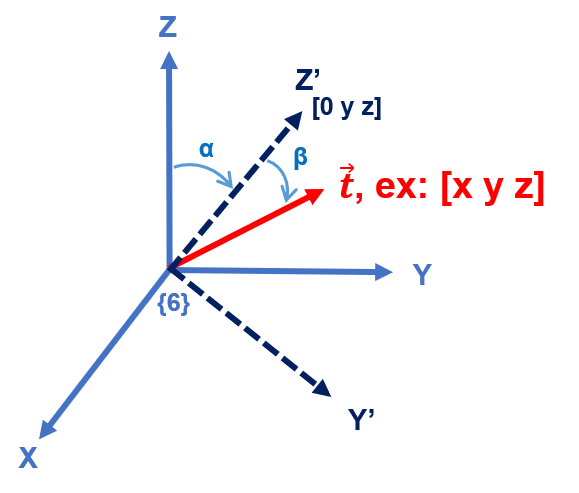
\includegraphics[width=0.8\linewidth]{../Images/rot_inf.png}
\end{center}
\caption{
Illustration of finding rotation matrix
}
\end{figure} 
Because we hope for sending z axis command to achieve tool insertion, we should align original Z axis to the target vector. Therefore, Z axis alignment without other restrictions will produce many solutions. We choose one of solutions to align Z axis to the target vector. According to the figure, we assume the target vector is [1,1,1], whose projection to YZ frame is [0,1,1]. First, we rotate $\alpha$ degree around X axis to make original Z axis align the projection [0,1,1]. Next, we rotate $\beta$ degree around Y' axis and finally align original Z axis to the target vector [1,1,1]. 
\begin{equation}
\begin{split}
\ ^T_6R = R_x\left(\alpha \right) R_y\left(\beta \right)  
\end{split}
\end{equation}
where $\alpha$ and $\beta$ are Euler angles equivalent to the command demand.

\section{Gravity Compensation}
\begin{equation*}
\begin{split}
\left\{\begin{matrix}
G_x = F_x - F_{x0}\\ 
G_z = F_y - F_{y0}\\ 
G_y = F_z - F_{z0}\\ 
M_{gx} = M_x - F_{x0}\\ 
M_{gy} = M_y - F_{y0}\\ 
M_{gz} = M_z - F_{z0}
\end{matrix}\right.	\\
%----------------------------------------------------------------------------------------------------------------------------
\left\{\begin{matrix}
M_{gx} = G_z \cdot y - G_y \cdot z\\ 
M_{gy} = G_x \cdot z - G_z \cdot x\\ 
M_{gz} = G_y \cdot x - G_x \cdot y
\end{matrix}\right.\\
%----------------------------------------------------------------------------------------------------------------------------
\begin{bmatrix}
M_x\\
M_y\\
M_z
\end{bmatrix}
=
\begin{bmatrix}
0		&F_z	&-F_y	&1	&0	&0\\
-F_z	&0		&F_x	&0	&1	&0\\
F_y		&-F_x	&0		&0	&0	&1
\end{bmatrix}
\begin{bmatrix}
x\\
y\\
z\\
k_1\\
k_2\\
k_3
\end{bmatrix}\\
%---------------------------------------------------------------------------------------------------------------------------
\left\{\begin{matrix}
k_1 = M_{x0} + F_{y0} \cdot z - F_{z0} \cdot y\\
k_2 = M_{y0} + F_{z0} \cdot x - F_{x0} \cdot z\\
k_3 = M_{z0} + F_{x0} \cdot y - F_{y0} \cdot x
\end{matrix}\right.\\
\end{split}
\end{equation*}

\begin{equation*}
\begin{split}
\begin{bmatrix}
cos\theta	&sin\theta	&0\\
-sin\theta	&cos\theta	&0\\
0			&0			&1	
\end{bmatrix}
\begin{bmatrix}
r_{00}	&r_{01}	&r_{02}\\
r_{10}	&r_{11}	&r_{12}\\
r_{20}	&r_{21}	&r_{22}
\end{bmatrix}
\begin{bmatrix}
0\\
0\\
-G
\end{bmatrix}
+
\begin{bmatrix}
F_{x0}\\
F_{y0}\\
F_{z0}
\end{bmatrix}
=
\begin{bmatrix}
F_x\\
F_y\\
F_z
\end{bmatrix}
\end{split}
\end{equation*}

\begin{equation*}
\begin{split}
\begin{bmatrix}
-r_{02}		&-r_{12}	&0			&1	&0	&0\\
-r_{12}		&r_{02}		&0			&0	&1	&0\\
0			&0			&-r_{22}	&0	&0	&1
\end{bmatrix}
\begin{bmatrix}
Gcos\theta\\
Gsin\theta\\
G\\
F_{x0}\\
F_{y0}\\
F_{z0}
\end{bmatrix}
=
\begin{bmatrix}
F_x\\
F_y\\
F_z
\end{bmatrix}
\end{split}
\end{equation*}
\begin{equation*}
\begin{split}
\left\{\begin{matrix}
F_{ex} = F_x - F_{x0} - G_x\\
F_{ey} = F_y - F_{y0} - G_y\\
F_{ez} = F_z - F_{z0} - G_z\\
M_{ex} = M_x - M_{x0} - M_{gx}\\
M_{ey} = M_y - M_{y0} - M_{gy}\\
M_{ez} = M_z - M_{z0} - M_{gz}\\
\end{matrix}\right.\\
%---------------------------------------------------------------------------------------------------------------------------
\left\{\begin{matrix}
G_x = -Gcos\theta r_{13} - Gsin\theta r_{23}\\
G_y =  Gsin\theta r_{13} - Gcos\theta r_{23}\\
G_z = -Gr_{33}
\end{matrix}\right.\\
%---------------------------------------------------------------------------------------------------------------------------
\theta = acos\left(\frac{Gcos\theta }{G}\right)\ or\ \theta = asin\left(\frac{Gsin\theta }{G}\right)                
\end{split}
\end{equation*}

\section{Admittance Control based on F/T Sensor}
Admittance control make the robot move like a spring-mass-damper system. Forces and torques can be mapped into the movements such as position or velocity. Therefore, Admittance control allows an robot arm to cooperate with human in a safe work environment. However, Meca500 is an industrial robot arm without admittance control, so we combine it with F/T sensor to enable this function. This combination make Meca500 like a cooperative robot arm. Whereas it's worth noting that the function is triggered by the end effector mounted on F/T sensor instead of each wrist of the robot arm.\\
A standard equation of admittance control is shown as Eq \ref{eq:adm}. The values we obtain from the F/T sensor are $\left[F_x, F_y, F_z,\tau _x, \tau _y, \tau _z \right]$, whose forces $ \left[F_x, F_y, F_z\right]$ are related to the translations $ \left[x, y, z\right]$ and torques $ \left[\tau _x, \tau _y, \tau _z\right]$ are related to the axis angle $ \left[\theta _x,\theta _y,\theta _z\right]$
\begin{equation}
\label{eq:adm}
\begin{split}
\begin{bmatrix}
x \\
y \\
z \\
\theta _x \\
\theta _y \\
\theta _z \\
\end{bmatrix}
=
\frac{1}{MS^2+BS+K}
\begin{bmatrix}
fx \\
fy \\
fz \\
\tau x \\
\tau y \\
\tau z \\
\end{bmatrix}
\end{split}
\end{equation}

\begin{equation*}
\begin{split}
&\begin{bmatrix}
\theta _x \\
\theta _y \\
\theta _z \\
\end{bmatrix}
=
_1^0\textrm{R}
\begin{bmatrix}
0 \\ 
0 \\ 
\theta _1\\
\end{bmatrix}
+
_1^0\textrm{R}
\begin{bmatrix}
0 \\ 
0 \\ 
\theta _2\\
\end{bmatrix}
+
_1^0\textrm{R}
\begin{bmatrix}
0 \\ 
0 \\ 
\theta _0\\
\end{bmatrix}
+
_1^4\textrm{R}
\begin{bmatrix}
0 \\ 
0 \\ 
\theta _0\\
\end{bmatrix}
+
_1^0\textrm{R}
\begin{bmatrix}
0 \\ 
0 \\ 
\theta _2\\
\end{bmatrix}
+
_1^2\textrm{R}
\begin{bmatrix}
0 \\ 
0 \\ 
\theta _2\\
\end{bmatrix}\\
%----------------------------------------------------------------------------------------------------------------------------
&\begin{bmatrix}					
\dot{x} \\ 
\dot{y} \\ 
\dot{z}\\ 
\dot{\theta _x} \\ 
\dot{\theta _y} \\ 
\dot{\theta _z}
\end{bmatrix}
=
\begin{bmatrix}
\dot{x} \\ 
\dot{y} \\ 
\dot{z}\\ 
w_x \\ 
w_y \\ 
w_z
\end{bmatrix}
=
J_g
\begin{bmatrix}
\dot{\theta _1} \\ 
\dot{\theta _2} \\ 
\dot{\theta _3} \\ 
\dot{\theta _4} \\ 
\dot{\theta _5} \\ 
\dot{\theta _6} \\ 
\end{bmatrix}	\\
%----------------------------------------------------------------------------------------------------------------------------
&J_g = 							
\begin{bmatrix}
J_{\vec{v}}\\ 
J_{\vec{w}} \\ 
\end{bmatrix}
\begin{bmatrix}
\dot{x} \\ 
\dot{y} \\ 
\dot{z}\\ 
\dot{\alpha} \\ 
\dot{\beta} \\ 
\dot{\gamma}
\end{bmatrix}
=
J_a
\begin{bmatrix}
\dot{\theta _1} \\ 
\dot{\theta _2} \\ 
\dot{\theta _3} \\ 
\dot{\theta _4} \\ 
\dot{\theta _5} \\ 
\dot{\theta _6} \\ 
\end{bmatrix}
\begin{bmatrix}
w_x \\
w_y \\ 
w_z
\end{bmatrix}
=
J_{we}
\begin{bmatrix}
\dot{\alpha } \\ 
\dot{\beta } \\
\dot{\gamma } \\
\end{bmatrix}\\
%----------------------------------------------------------------------------------------------------------------------------
&J_{we} =				
\begin{bmatrix}
1 & 0 & S_\beta \\ 
0 & C_\alpha & -S_\alpha C_\beta \\ 
0 & S_\alpha & C_\alpha C_\beta
\end{bmatrix}
\begin{bmatrix}
\theta _x \\ 
\theta _y \\ 
\theta _z
\end{bmatrix}
=
\begin{bmatrix}
\alpha \\ 
0\\ 
0
\end{bmatrix}
+
R_x(\alpha)
\begin{bmatrix}
0 \\ 
\beta \\ 
0
\end{bmatrix}
+
R_x(\alpha)R_y(\beta) \\
%----------------------------------------------------------------------------------------------------------------------------   
&\begin{bmatrix}
0 \\ 
0\\ 
\gamma
\end{bmatrix}
=
\begin{bmatrix}
1 & 0 & S_\beta \\ 
0 & C_\alpha & -S_\alpha C_\beta \\ 
0 & S_\alpha & C_\alpha C_\beta
\end{bmatrix}
\begin{bmatrix}
\alpha \\ 
\beta\\ 
\gamma
\end{bmatrix}\\
%----------------------------------------------------------------------------------------------------------------------------
&\begin{bmatrix}				
\dot{x} \\
\dot{y} \\
\dot{z} \\
w_x \\ 
w_y \\ 
w_z
\end{bmatrix}
=
\begin{bmatrix}
I_{3\times 3} & 0_{3\times 3}\\
0_{3\times 3} & J_{we}
\end{bmatrix}
\begin{bmatrix}
\dot{x} \\
\dot{y} \\
\dot{z} \\
\dot{\alpha} \\ 
\dot{\beta} \\ 
\dot{\gamma} 
\end{bmatrix}\\
%----------------------------------------------------------------------------------------------------------------------------					
&Jg = 							
\begin{bmatrix}
I_{3\times 3} & 0_{3\times 3}\\
0_{3\times 3} & J_{we}
\end{bmatrix}
Ja
\end{split}
\end{equation*}
\section{Reference Frame Changing}
\begin{equation*}
\begin{split}
&M_q = r_qF\\
&M_p = r_pF+\overrightarrow{qp}\times F_p\\
&M_q = M_p + \vec{qp} \times F_p\\
&\begin{bmatrix}
F_q\\ 
M_q
\end{bmatrix}
_{S2}
=
\begin{bmatrix}
I_{3 \times 3} & 0\\ 
^{S_2}[S_{1org}-S_{2org}]_x & I_{3 \times 3}
\end{bmatrix}
\begin{bmatrix}
_{S1}^{S2}\textrm{R} & 0\\ 
0 & _{S1}^{S2}\textrm{R}
\end{bmatrix}
\begin{bmatrix}
F_p\\ 
M_p
\end{bmatrix}
_{S1}\\
&M_q = r_qF\\
&M_p = r_pF+ ^{S_2}[S_{1org}-S_{2org}]_x\times F_p\\
&M_q = M_p + ^{S_2}[S_{1org}-S_{2org}]_x \times F_p\\
&^{S_2}_{S_1}T = 
\begin{bmatrix}
^{S_2}_{S_1}R   & ^{S2}\vec{P}_{s_{1 org} }\\ 
0               & 1
\end{bmatrix}
=
\begin{bmatrix}
I & ^{S2}\vec{P}_{s_{1 org} }\\ 
0 & 1
\end{bmatrix}
\begin{bmatrix}
^{S_2}_{S_1}R & 0\\ 
0 & 1
\end{bmatrix}\\
&^{S_2}\vec{P}_{s_{1 org} } = -^{S_2}_{S_1}R \cdot ^{S_1}\vec{P}_{s_{2 org}}\\
\end{split}
\end{equation*}
\section{Appendix}
\subsection{Forward Kinematics}\label{appendix:forward}
\begin{equation*}
\begin{split}
^0_6\text{T} =
^0_1\text{T} \cdot ^1_2\text{T} \cdot ^2_3\text{T} \cdot ^3_4\text{T} \cdot ^4_5\text{T} \cdot ^5_6\text{T} =
\begin{bmatrix}
^0_6\text{R}_{3\times 3} 	&^0\vec{P}_{6org}\\
0_{1\times 3}				&1\\
\end{bmatrix}
=
\begin{bmatrix}
^0_6\text{T}_{00} 	&^0_6\text{T}_{01}	&^0_6\text{T}_{02}	& ^0_6\text{T}_{03}\\
^0_6\text{T}_{10} 	&^0_6\text{T}_{11}	&^0_6\text{T}_{12}	& ^0_6\text{T}_{13}\\
^0_6\text{T}_{20} 	&^0_6\text{T}_{21}	&^0_6\text{T}_{22}	& ^0_6\text{T}_{23}\\
0					&0					&0					&1\\
\end{bmatrix}
\end{split}
\end{equation*}
\begin{equation*}
\begin{split}
^0_6\mathbf{T}_{00} = &- S_6(C_4S_1 + S_4(C_1S_3-C_2 - C_1C_3S_2)) - C_6(C_5(S_1S_4 - C_4(C_1S_3-C_2 - C_1C_3S_2))\\
					& - S_5(C_1C_3-C_2 + C_1S_2S_3))\\
^0_6\text{T}_{01} = &S_6(C_5(S_1S_4 - C_4(C_1S_3-C_2 - C_1C_3S_2)) - S_5(C_1C_3-C_2 + C_1S_2S_3))- C_6(C_4S_1\\
					& + S_4(C_1S_3-C_2 - C_1C_3S_2))\\
^0_6\text{T}_{02} = &- S_5(S_1S_4 - C_4(C_1S_3-C_2 - C_1C_3S_2)) - C_5(C_1C_3-C_2 + C_1S_2S_3)\\
^0_6\text{T}_{03} = &135C_1S_2 - 70S_5(S_1S_4 - C_4(C_1S_3-C_2 - C_1C_3S_2)) - 70C_5(C_1C_3-C_2 + C_1S_2S_3)\\
					& - 120C_1C_3-C_2 - 120C_1S_2S_3 - 38C_1S_3-C_2 + 38C_1C_3S_2\\
^0_6\text{T}_{10} = &S_6(C_1C_4 + S_4(C_3S_2S_1 - S_1S_3-C_2)) + C_6(C_5(C_1S_4 - C_4(C_3S_2S_1 - S_1S_3-C_2))\\
					& + S_5(C_3S_1-C_2 + S_2S_1S_3))\\
^0_6\text{T}_{11} = &C_6(C_1C_4 + S_4(C_3S_2S_1 - S_1S_3-C_2)) - S_6(C_5(C_1S_4 - C_4(C_3S_2S_1 - S_1S_3-C_2))\\
					& + S_5(C_3S_1-C_2 + S_2S_1S_3))\\
^0_6\text{T}_{12} = &S_5(C_1S_4 - C_4(C_3S_2S_1 - S_1S_3-C_2)) - C_5(C_3S_1-C_2 + S_2S_1S_3)\\
^0_6\text{T}_{13} = &135S_2S_1 + 70S_5(C_1S_4 - C_4(C_3S_2S_1 - S_1S_3-C_2)) - 70C_5(C_3S_1-C_2 + S_2S_1S_3)\\
					& + 38C_3S_2S_1 - 120C_3S_1-C_2 - 120S_2S_1S_3 - 38S_1S_3-C_2\\
^0_6\text{T}_{20} = &C_6(S_5(C_3S_2 - S_3-C_2) + C_4C_5(C_3-C_2 + S_2S_3)) - S_4S_6(C_3-C_2 + S_2S_3)\\
^0_6\text{T}_{21} = &- S_6(S_5(C_3S_2 - S_3-C_2) + C_4C_5(C_3-C_2 + S_2S_3)) - C_6S_4(C_3-C_2 + S_2S_3)\\
^0_6\text{T}_{22} = &C_4S_5(C_3-C_2 + S_2S_3) - C_5(C_3S_2 - S_3-C_2)\\
^0_6\text{T}_{23} = &120S_3-C_2 - 120C_3S_2 - 38C_3-C_2 - 38S_2S_3 - 135-C_2 - 70C_5(C_3S_2 - S_3-C_2)\\
					& + 70C_4S_5(C_3-C_2 + S_2S_3) + 135\\
\end{split}
\end{equation*}
\subsection{Jacobian matrix}\label{appendix:jacobian}

\begin{equation*}
\begin{split}
J_{g0,00} =\  &120S_1S_2S_3 - 38C_2S_1S_3 - 38C_3S_1S_2 - 70C_1S_4S_5 - 135S_1S_2 - 120C_2C_3S_1\\
         	  &- 70C_2C_3C_5S_1 + 70C_5S_1S_2S_3  + 70C_2C_4S_1S_3S_5 + 70C_3C_4S_1S_2S_5\\
J_{g0,01} =\  &-C_1(120C_2S_3 - 38C_2C_3 - 135C_2 + 120C_3S_2 + 38S_2S_3 + 70C_2C_5S_3 \\
         	  &+ 70C_3C_5S_2 + 70C_2C_3C_4S_5 - 70C_4S_2S_3S_5)\\
J_{g0,02} =\  &-2C_1(60C_2S_3 - 19C_2C_3 + 60C_3S_2 + 19S_2S_3 + 35C_2C_5S_3 + 35C_3C_5S_2\\ 
         	  &+ 35C_2C_3C_4S_5 - 35C_4S_2S_3S_5)\\
J_{g0,03} =\  &70S_5(C_1C_2S_3S_4 - C_4S_1 + C_1C_3S_2S_4)\\
J_{g0,04} =\  &- 70C_5(S_1S_4 + C_1C_2C_4S_3 + C_1C_3C_4S_2) - 70C_{23}C_1S_5\\
J_{g0,05} =\  &0\\
J_{g0,10} =\  &135C_1S_2 - 120C_1S_2S_3 - 70S_1S_4S_5 + 120C_1C_2C_3 + 38C_1C_2S_3 + 38C_1C_3S_2 \\
		 	  &+ 70C_1C_2C_3C_5 - 70C_1C_5S_2S_3 - 70C_1C_2C_4S_3S_5 - 70C_1C_3C_4S_2S_5\\
J_{g0,11} =\  &-S_1(120C_2S_3 - 38C_2C_3 - 135C_2 + 120C_3S_2 + 38S_2S_3 + 70C_2C_5S_3\\
		   	  &+ 70C_3C_5S_2 + 70C_2C_3C_4S_5 - 70C_4S_2S_3S_5)\\
J_{g0,12} =\  &-2S_1(60C_2S_3 - 19C_2C_3 + 60C_3S_2 + 19S_2S_3 + 35C_2C_5S_3 + 35C_3C_5S_2 \\ 
		 	  &+ 35C_2C_3C_4S_5 - 35C_4S_2S_3S_5)\\
J_{g0,13} =\  &70S_5(C_1C_4 + C_2S_1S_3S_4 + C_3S_1S_2S_4)\\
J_{g0,14} =\  &- 70C_5(C_2C_4S_1S_3 - C_1S_4 + C_3C_4S_1S_2) - 70C_{23}S_1S_5\\
J_{g0,15} =\  &0\\
J_{g0,20} =\  &0\\
J_{g0,21} =\  &120S_2S_3 - 120C_2C_3 - 38C_2S_3 - 38C_3S_2 - 135S_2 + 70C_5S_2S_3 - 70C_2C_3C_5\\
		 	  &+ 70C_2C_4S_3S_5 + 70C_3C_4S_2S_5\\
J_{g0,22} =\  &120S_2S_3 - 38C_2S_3 - 38C_3S_2 - 120C_2C_3 + 70C_5S_2S_3 - 70C_2C_3C_5 + 70C_2C_4S_3S_5\\
		 	  &+ 70C_3C_4S_2S_5\\
J_{g0,23} =\  &70C_{23}S_4S_5\\
J_{g0,24} =\  &70S_{23}S_5 - 70C_{23}C_4C_5\\
J_{g0,25} =\  &0\\
J_{g0,30} =\  &\theta _4S_1S_2S_3 - \theta _3C_1 - \theta _5C_1C_4 - \theta _4C_2C_3S_1 - \theta _6C_1S_4S_5 - \theta _2C_1 - \theta _6C_2C_3C_5S_1\\
		 	  &- \theta _5C_2S_1S_3S_4 - \theta _5C_3S_1S_2S_4 + \theta _6C_5S_1S_2S_3 + \theta _6C_2C_4S_1S_3S_5 + \theta _6C_3C_4S_1S_2S_5\\
J_{g0,31} =\  &\theta _5C_1C_2C_3S_4 - \theta _4C_1C_2S_3 - \theta _4C_1C_3S_2 - S_1 - \theta _6C_1C_2C_5S_3 - \theta _6C_1C_3C_5S_2\\
		 	  &- \theta _5C_1S_2S_3S_4 - \theta _6C_1C_2C_3C_4S_5 + \theta _6C_1C_4S_2S_3S_5\\
J_{g0,32} =\  &\theta _5C_1C_2C_3S_4 - \theta _4C_1C_2S_3 - \theta _4C_1C_3S_2 - S_1 - \theta _6C_1C_2C_5S_3 - \theta _6C_1C_3C_5S_2\\
			  &- \theta _5C_1S_2S_3S_4 - \theta _6C_1C_2C_3C_4S_5 + \theta _6C_1C_4S_2S_3S_5\\
J_{g0,33} =\  &\theta _5(S_1S_4 + C_1C_2C_4S_3 + C_1C_3C_4S_2) - C_1S_2S_3 + C_1C_2C_3 + \theta _6S_5(C_1C_2S_3S_4\\
			  &- C_4S_1 + C_1C_3S_2S_4)\\
J_{g0,34} =\  &- C_4S_1 - \theta _6(C_5(S_1S_4 - C_4(C_1S_3-C_2 - C_1C_3S_2)) - S_5(C_1C_3-C_2 + C_1S_2S_3))\\
			  &- S_4(C_1S_3-C_2 - C_1C_3S_2)\\
J_{g0,35} =\  &C_{23}C_1C_5 - S_5(S_1S_4 + C_1C_2C_4S_3 + C_1C_3C_4S_2)\\
\end{split}
\end{equation*}
\begin{equation*}
\begin{split}
J_{g0,40} =\  &\theta _4C_1C_2C_3 - \theta _3S_1 - \theta _5C_4S_1 - theta2S_1 - \theta _4C_1S_2S_3 - \theta _6S_1S_4S_5 + \theta _6C_1C_2C_3C_5\\
		 	  &+ \theta _5C_1C_2S_3S_4 + \theta _5C_1C_3S_2S_4 - \theta _6C_1C_5S_2S_3 - \theta _6C_1C_2C_4S_3S_5 - \theta _6C_1C_3C_4S_2S_5\\
J_{g0,41} =\  &C_1 - \theta _4C_2S_1S_3 - \theta _4C_3S_1S_2 + \theta _5C_2C_3S_1S_4 - \theta _6C_2C_5S_1S_3 - \theta _6C_3C_5S_1S_2 \\
		 	  &- \theta _5S_1S_2S_3S_4 - \theta _6C_2C_3C_4S_1S_5 + \theta _6C_4S_1S_2S_3S_5\\
J_{g0,42} =\  &C_1 - \theta _4C_2S_1S_3 - \theta _4C_3S_1S_2 + \theta _5C_2C_3S_1S_4 - \theta _6C_2C_5S_1S_3 - \theta _6C_3C_5S_1S_2\\
			  & - \theta _5S_1S_2S_3S_4\\
		 	  &- \theta _6C_2C_3C_4S_1S_5 + \theta _6C_4S_1S_2S_3S_5\\
J_{g0,43} =\  &\theta _5(C_2C_4S_1S_3 - C_1S_4 + C_3C_4S_1S_2) + \theta _6S_5(C_1C_4 + C_2S_1S_3S_4 + C_3S_1S_2S_4)\\
		 	  &- S_1S_2S_3 + C_2C_3S_1\\
J_{g0,44} =\  &C_1C_4 + S_{23}S_1S_4 - \theta _6C_{23}S_1S_5 + \theta _6C_1C_5S_4 - \theta _6C_2C_4C_5S_1S_3 - \theta _6C_3C_4C_5S_1S_2\\
J_{g0,45} =\  &C_{23}C_5S_1 - S_5(C_2C_4S_1S_3 - C_1S_4 + C_3C_4S_1S_2)\\
J_{g0,50} =\  &1\\
J_{g0,51} =\  &\theta _6S_{23}C_4S_5 - \theta _6C_{23}C_5 - \theta _5S_{23}S_4 - \theta _4C_{23}\\
J_{g0,52} =\  &\theta _6S_{23}C_4S_5 - \theta _6C_{23}C_5 - \theta _5S_{23}S_4 - \theta _4C_{23}\\
J_{g0,53} =\  &\theta _5C_2C_3C_4 - C_3S_2 - C_2S_3 - \theta _5C_4S_2S_3 + \theta _6C_2C_3S_4S_5 - \theta _6S_2S_3S_4S_5\\
J_{g0,54} =\  &\theta _6(S_{23}S_5 - C_{23}C_4C_5) + C_{23}S_4\\
J_{g0,55} =\  &- S_{23}C_5 - C_{23}C_4S_5\\
J_{g6,00} =\  &135C_4S_2S_6 + 120C_2C_3C_4S_6 + 70C_2C_3C_6S_4 + 38C_2C_4S_3S_6 + 38C_3C_4S_2S_6\\
			  &+ 135C_5C_6S_2S_4 - 120C_4S_2S_3S_6 - 70C_6S_2S_3S_4 - 70C_2S_3S_5S_6 - 70C_3S_2S_5S_6\\
			  &+ 70C_2C_3C_4C_5S_6 + 120C_2C_3C_5C_6S_4 + 38C_2C_5C_6S_3S_4 + 38C_3C_5C_6S_2S_4\\
			  &- 70C_4C_5S_2S_3S_6 - 120C_5C_6S_2S_3S_4\\
J_{g6,01} =\  &70C_4C_6 - 38C_6S_5 - 120S_4S_6 - 70C_5S_4S_6 + 135S_3S_4S_6 + 120C_4C_5C_6 - 135C_3C_6S_5\\
			  &- 135C_4C_5C_6S_3\\   
J_{g6,02} =\  &70C_4C_6 - 38C_6S_5 - 120S_4S_6 - 70C_5S_4S_6 + 120C_4C_5C_6\\
J_{g6,03} =\  &70S_5S_6\\
J_{g6,04} =\  &70C_6\\
J_{g6,05} =\  &0\\
J_{g6,10} =\  &135C_4C_6S_2 + 120C_2C_3C_4C_6 + 38C_2C_4C_6S_3 + 38C_3C_4C_6S_2 - 70C_2C_3S_4S_6\\
			  & - 120C_4C_6S_2S_3 - 70C_2C_6S_3S_5 - 70C_3C_6S_2S_5 - 135C_5S_2S_4S_6 + 70S_2S_3S_4S_6\\
			  & + 70C_2C_3C_4C_5C_6 - 120C_2C_3C_5S_4S_6 - 70C_4C_5C_6S_2S_3 - 38C_2C_5S_3S_4S_6\\
			  & - 38C_3C_5S_2S_4S_6 + 120C_5S_2S_3S_4S_6\\
J_{g6,11} =\  &38S_5S_6 - 120C_6S_4 - 70C_4S_6 + 135C_6S_3S_4 + 135C_3S_5S_6 - 120C_4C_5S_6 - 70C_5C_6S_4\\
			  & + 135C_4C_5S_3S_6\\
J_{g6,12} =\  &38S_5S_6 - 120C_6S_4 - 70C_4S_6 - 120C_4C_5S_6 - 70C_5C_6S_4\\
J_{g6,13} =\  &70C_6S_5\\
J_{g6,14} =\  &-70S_6\\
J_{g6,15} =\  &0\\
\end{split}
\end{equation*}
\end{CJK}
\end{document}